\chapter{AI in DevOps: CI/CD, Defects, and Estimation}\label{ch:devops}
\begin{center}\small\textit{DevOps closes the loop from commit to customer; AI makes the loop faster, safer, and more predictable.}\end{center}

\begin{quote}\small\textbf{From zero: no DevOps background assumed.} We build from ``what is CI/CD?'' through pipelines, feedback loops, and measurement before any model appears. Every formula is motivated by a picture.\end{quote}

\noindent\fbox{\parbox{\dimexpr\linewidth-2\fboxsep-2\fboxrule}{%
\textbf{Learning Outcomes.} After this chapter you will be able to (1)~sketch a CI/CD pipeline and its quality gates; (2)~explain where AI plugs into DevOps; (3)~formulate defect prediction as supervised learning; (4)~contrast algorithmic and ML-based effort estimation; (5)~measure DevOps impact with DORA-style metrics.}}
\vspace{0.4em}

% ============================================================
\section{Intuition: The DevOps Loop}\label{sec:devops-intuition}
Traditional development threw code ``over the wall'' to operations. \textbf{DevOps} tears down the wall: one cross-functional team owns code, build, test, deploy, monitor, and learn --- as a single loop. Two practices automate the loop:

\begin{itemize}[leftmargin=1.2em, itemsep=0.3em]
  \item \textbf{Continuous Integration (CI)} --- every commit triggers an automated pipeline: compile, unit-test, lint, security scan, and package. Failures are reported in minutes, not days.
  \item \textbf{Continuous Delivery/Deployment (CD)} --- every green build is automatically staged, and (with deployment) released to users behind feature flags and canaries.
\end{itemize}

Lead time shrinks from weeks to hours. The cost is complexity: more automation means more logs, more signals, and more decisions about \emph{what} to test, \emph{where} bugs lurk, and \emph{how long} work will take. Those decisions are where AI earns its keep.

% ============================================================
\section{AI Across the Pipeline}\label{sec:ai-pipeline}
Think of the pipeline as an assembly line with inspectors. AI inspectors can stand at every station:

\begin{center}
\begin{tikzpicture}[font=\scriptsize, >=Stealth, scale=0.86, stage/.style={draw, rounded corners, minimum width=1.95cm, minimum height=1.0cm, align=center}]
  \node[stage, fill=blue!12] (commit) at (0,0) {Commit\\{\tiny git push}};
  \node[stage, fill=green!12] (build) at (2.85,0) {Build\\{\tiny compile}};
  \node[stage, fill=orange!14] (test) at (5.7,0) {Test\\{\tiny unit / e2e}};
  \node[stage, fill=violet!12] (sec) at (8.55,0) {Security\\{\tiny SAST/DAST}};
  \node[stage, fill=red!10] (deploy) at (11.4,0) {Deploy\\{\tiny canary}};
  \node[stage, fill=gray!14] (monitor) at (11.4,-1.7) {Monitor\\{\tiny logs, metrics}};
  \draw[->, thick, blue!60!black] (commit) -- (build);
  \draw[->, thick, blue!60!black] (build) -- (test);
  \draw[->, thick, blue!60!black] (test) -- (sec);
  \draw[->, thick, blue!60!black] (sec) -- (deploy);
  \draw[->, thick, blue!60!black] (deploy) -- (monitor);
  % AI badges
  \node[font=\tiny, fill=yellow!12, draw, rounded corners, inner sep=2pt, align=center] at (2.85,1.2) {AI: build\\failure pred.};
  \node[font=\tiny, fill=yellow!12, draw, rounded corners, inner sep=2pt, align=center] at (5.7,1.2) {AI: test\\selection};
  \node[font=\tiny, fill=yellow!12, draw, rounded corners, inner sep=2pt, align=center] at (8.55,1.2) {AI: vuln\\ranking};
  \node[font=\tiny, fill=yellow!12, draw, rounded corners, inner sep=2pt, align=center] at (11.4,1.05) {AI: canary\\analysis};
  \node[font=\tiny, fill=yellow!12, draw, rounded corners, inner sep=2pt, align=center] at (11.4,-2.9) {AI: anomaly\\detection};
  % feedback loop
  \draw[->, thick, dashed, gray!60!black, bend left=20] (monitor.west) to node[below, font=\tiny, fill=white, inner sep=1pt] {feedback / auto-rollback} (commit.south);
  \node[font=\tiny, text=gray!60!black] at (5.7,-1.05) {quality gates \quad $\leftarrow$ \quad risk scores};
\end{tikzpicture}
\end{center}

Concrete AI insertions that teams actually ship:

\begin{enumerate}[leftmargin=1.2em, itemsep=0.3em]
  \item \textbf{Build-failure prediction} --- before running the full pipeline, predict $P(\text{fail}\mid\text{diff})$ from diff size, churn, author history, and files touched; skip or prioritise.
  \item \textbf{Test selection \& prioritisation} --- run the 5\% of tests most likely to fail first (based on dependency graph + recent failures), so developers get signal in seconds.
  \item \textbf{Log anomaly detection} --- learn normal log templates (Drain, Spell) then flag rare templates or sequences that precede incidents.
  \item \textbf{Canary analysis} --- compare canary vs.\ baseline on latency/error metrics with statistical or ML-based change-point detection; auto-roll back on regression.
\end{enumerate}

All four share a pattern: learn from history, score the present, and act (reorder, skip, or block) with an explainable reason.

% ============================================================
\section{Defect Prediction: Will This Change Break?}\label{sec:defect-pred}
\textbf{Defect prediction} asks: given a file, commit, or pull request, what is the probability it introduces a bug? Early work predicted at \emph{release} granularity (``which files will have post-release defects?''); modern work predicts at \emph{commit} or \emph{just-in-time} granularity, which is far more actionable.

Formally, for each instance $x_i$ (a file or commit) with label $y_i\in\{0,1\}$ (1 = buggy), learn $f:\mathcal{X}\to[0,1]$ where $f(x_i)\approx P(y_i=1\mid x_i)$. Training data come from linking bug-fix commits back to the commits that introduced the bug (SZZ algorithm and variants --- noisy but standard).

Features fall into three families:

\begin{center}
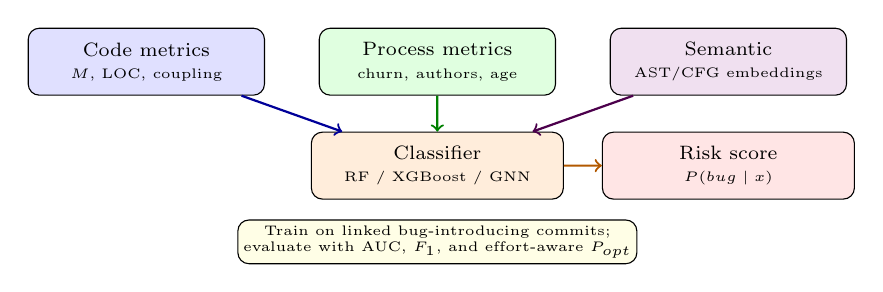
\begin{tikzpicture}[font=\scriptsize, scale=0.88]
  \node[draw, fill=blue!12, rounded corners, minimum width=3.0cm, minimum height=0.85cm, align=center] (code) at (0,0) {Code metrics\\{\tiny $M$, LOC, coupling}};
  \node[draw, fill=green!12, rounded corners, minimum width=3.0cm, minimum height=0.85cm, align=center] (proc) at (4.2,0) {Process metrics\\{\tiny churn, authors, age}};
  \node[draw, fill=violet!12, rounded corners, minimum width=3.0cm, minimum height=0.85cm, align=center] (sem) at (8.4,0) {Semantic\\{\tiny AST/CFG embeddings}};
  \node[draw, fill=orange!14, rounded corners, minimum width=3.2cm, minimum height=0.85cm, align=center] (model) at (4.2,-1.5) {Classifier\\{\tiny RF / XGBoost / GNN}};
  \node[draw, fill=red!10, rounded corners, minimum width=3.2cm, minimum height=0.85cm, align=center] (out) at (8.4,-1.5) {Risk score\\{\tiny $P(\text{bug}\mid x)$}};
  \draw[->, thick, blue!60!black] (code) -- (model);
  \draw[->, thick, green!50!black] (proc) -- (model);
  \draw[->, thick, violet!60!black] (sem) -- (model);
  \draw[->, thick, orange!70!black] (model) -- (out);
  \node[font=\tiny, fill=yellow!10, draw, rounded corners, inner sep=2pt, align=center] at (4.2,-2.6) {Train on linked bug-introducing commits;\\evaluate with AUC, $F_1$, and effort-aware $P_{\text{opt}}$};
\end{tikzpicture}
\end{center}

Process metrics often beat code metrics alone: a file with high churn touched by many authors is riskier than a complex but stable file. Semantic embeddings (CodeBERT, GraphCodeBERT over AST/CFG) add further gains, especially for cross-project prediction where raw metric distributions shift.

Handling imbalance matters: only 10--20\% of commits are buggy, so train with class weighting, SMOTE, or focal loss, and report \textbf{AUC} and \textbf{effort-aware} measures ($P_{\text{opt}}$, $\text{AUCEC}$) that ask ``how many bugs do we find if we inspect the top 20\% riskiest code?'' rather than raw accuracy.

\begin{example}[Just-in-time defect prediction in Python]\label{ex:defect}
\begin{lstlisting}[language=Python,caption={JIT defect prediction with process + code features and XGBoost.},label={lst:defect}]
import pandas as pd
from sklearn.model_selection import train_test_split
from sklearn.metrics import roc_auc_score, classification_report
from xgboost import XGBClassifier

# Toy dataset: each row is a commit; label 1 = introduced a bug (via SZZ)
data = pd.DataFrame({
    "churn":        [12, 180, 5, 220, 30, 90, 15, 300, 8, 150],
    "num_authors":  [1, 4, 1, 5, 2, 3, 1, 6, 1, 3],
    "cyclomatic":   [3, 18, 2, 22, 5, 12, 4, 25, 2, 14],
    "file_age_days":[200, 30, 400, 15, 180, 60, 300, 10, 500, 45],
    "buggy":        [0, 1, 0, 1, 0, 1, 0, 1, 0, 1],
})
X = data[["churn","num_authors","cyclomatic","file_age_days"]]
y = data["buggy"]
Xtr, Xte, ytr, yte = train_test_split(X, y, test_size=0.3, random_state=42, stratify=y)

clf = XGBClassifier(use_label_encoder=False, eval_metric="logloss",
                    scale_pos_weight=1.2, max_depth=3, n_estimators=80)
clf.fit(Xtr, ytr)
proba = clf.predict_proba(Xte)[:, 1]
print(f"AUC: {roc_auc_score(yte, proba):.2f}")
print(classification_report(yte, (proba > 0.5).astype(int)))
# Actionable use: rank PRs by proba, inspect top-k
ranked = sorted(zip(Xte.index, proba), key=lambda x: -x[1])
print("Inspect first:", ranked[:2])
\end{lstlisting}
\end{example}

Deployment tip: surface the score in the PR as ``risk: high (churn 220, $M$=22, 5 authors)'' and offer to auto-add reviewers or require extra tests --- developers accept guidance that explains \emph{why}.

% ============================================================
\section{Effort Estimation: How Long Will It Take?}\label{sec:effort}
Estimation is notorious: Brooks's law, optimism bias, and shifting scope conspire against it. Two traditions meet here.

\textbf{Algorithmic models} encode expert judgement as formulas. The classic is COCOMO (Boehm, 1981):
\[
  \text{Effort (person-months)} = a \cdot (\text{KLOC})^{b}\cdot \prod_i \text{EM}_i,
\]
where $a,b$ depend on project class and $\text{EM}_i$ are effort multipliers (required reliability, analyst capability, tool use, \dots). COCOMO II refines this with scale factors (precedence, team cohesion) and reuse. These models are interpretable but need careful calibration per organisation.

\textbf{ML-based estimation} learns from history: given features (story points, function points, team velocity, textual description embeddings, dependency graph), regress to actual effort. Modern variants fine-tune language models on issue text + labels (hours or story points), or use analogy-based reasoning (find $k$ nearest past issues and average their effort).

Evaluation must respect time: train on past sprints, test on future ones (no shuffling). Report \textbf{MAE}, \textbf{MMRE} $=\frac1n\sum|(\hat y_i-y_i)/y_i|$, and \textbf{PRED(25)} $=$ fraction within 25\% of true effort. No model beats seasoned judgement by a huge margin; the win is consistency and calibration --- ML estimates come with a predicted interval, so planning can use $P_{50}$ and $P_{90}$ rather than a point guess.

\begin{center}
\begin{tikzpicture}[font=\scriptsize, >=Stealth, scale=0.88]
  \draw[->, thick] (0,0) -- (7,0) node[right] {Time (sprints)};
  \draw[->, thick] (0,0) -- (0,2.8) node[above] {Effort (person-days)};
  % true effort dots
  \foreach \x/\y in {0.7/1.0, 1.5/0.6, 2.3/1.8, 3.1/1.2, 3.9/2.2, 4.7/1.6, 5.5/2.0, 6.2/1.4} {
    \fill[blue!70!black] (\x,\y) circle (2.2pt);
  }
  % predicted band
  \fill[orange!15] (0.4,0.5) -- (6.5,1.0) -- (6.5,1.9) -- (0.4,1.4) -- cycle;
  \draw[thick, orange!60!black] (0.4,0.95) -- (6.5,1.45) node[above right, font=\tiny, fill=white, inner sep=1pt] {ML prediction $+$ interval};
  \draw[dashed, gray!50!black] (0.4,0.4) -- (6.5,0.9);
  \draw[dashed, gray!50!black] (0.4,1.5) -- (6.5,2.0);
  \node[font=\tiny, fill=blue!10, draw, rounded corners, inner sep=2pt, align=center] at (3.2,2.5) {Dots = actual; band = $P_{10}$--$P_{90}$};
  \node[font=\tiny, text=green!50!black] at (1.8,2.2) {Use $P_{50}$ for plan, $P_{90}$ for buffer};
\end{tikzpicture}
\end{center}

% ============================================================
\section{Worked Example: Prioritising Tests with History}\label{sec:devops-worked}
Suppose nightly CI runs 2\,000 tests but developers need feedback in under 3\,min. Historical data show that 15 tests fail on 40\% of buggy PRs. A simple AI prioritiser scores each test $t$ by
\[
  s(t) = \alpha\cdot \text{fail\_rate}(t) + \beta\cdot \text{cochange}(t,\Delta) + \gamma\cdot \text{distance}(t,\Delta),
\]
where $\text{cochange}$ is how often $t$ and changed files $\Delta$ were modified together and $\text{distance}$ is graph distance in the dependency graph. Sorting by $s(t)$ and running the top 5\% first catches 70\% of failures within the first minute. A second listing adds confidence:

\begin{lstlisting}[language=Python,caption={Ranking tests by failure history and co-change.},label={lst:test-rank}]
import pandas as pd

tests = pd.DataFrame({
    "test": ["t_login","t_export","t_auth","t_report","t_api"],
    "fail_rate": [0.40, 0.05, 0.30, 0.02, 0.10],
    "cochange":  [0.8,  0.1,  0.6,  0.0,  0.4 ],
    "distance":  [1,    4,    1,    5,    2   ],  # graph hops to changed file
})
alpha, beta, gamma = 0.5, 0.3, 0.2
tests["score"] = alpha*tests.fail_rate + beta*tests.cochange - gamma*(tests.distance/5)
print(tests.sort_values("score", ascending=False)[["test","score"]].to_string(index=False))
# Run top-2 first: t_login and t_auth catch most signal quickly.
\end{lstlisting}

% ============================================================
\section{Common Pitfalls}\label{sec:devops-pitfalls}
\begin{itemize}[leftmargin=1.2em, itemsep=0.3em]
  \item \textbf{Leaking the future.} Training defect prediction on data that includes the bug-fix commit itself inflates AUC. Split strictly by time: train on sprints 1--8, validate on 9, test on 10.
  \item \textbf{Optimising the wrong metric.} AUC rewards ranking but ignores inspection cost. Always report effort-aware $P_{\text{opt}}$ or Cost-Effectiveness alongside AUC.
  \item \textbf{Flaky tests as signal.} A test that flakes randomly will earn a high fail rate and dominate prioritisation. De-flake first or down-weight known flaky tests.
  \item \textbf{Estimation without intervals.} A point estimate of ``5 days'' that lands at 9 days breaks a sprint. Report $P_{50}$ and $P_{90}$ so planners can buffer realistically.
\end{itemize}

% ============================================================
\section{Closing the Loop: Measurement that Matters}\label{sec:measure}
Gates and predictions are only useful if they improve outcomes. The DORA framework (Forsgren et al.) gives four team-level yardsticks: \textbf{deployment frequency}, \textbf{lead time for changes}, \textbf{change failure rate}, and \textbf{mean time to recovery (MTTR)}. AI interventions should move at least one of these without harming the others --- e.g., test prioritisation should raise deployment frequency (faster signal) without raising change failure rate (missed bugs). Always A/B the change: enable the ranker for half the PRs, compare escaped defects and review latency.

% ============================================================
\section{Chapter Summary}\label{sec:devops-summary}
DevOps is a loop; AI shortens it. In CI/CD, ML reorders and prunes work so humans see what matters first. Defect prediction scores each change by $P(\text{bug}\mid x)$ using code, process, and semantic signals; effort estimation regresses from history to intervals that planning can actually use. Measure success with DORA metrics, not offline AUC alone.

% ============================================================
\section{Exercises}\label{sec:devops-ex}
\begin{enumerate}[label=E7.\arabic*, leftmargin=*, itemsep=0.75em]
  \item \textbf{Pipeline mapping.} Map each AI insertion from Sec.~\ref{sec:ai-pipeline} to a DORA metric it should improve. For one, state a confound that could make the metric improve without real quality gain.
  \item \textbf{Defect features.} You have only code metrics ($M$, LOC). A colleague proposes adding \emph{number of authors} and \emph{churn}. Explain why process features often beat code features, and design an experiment to test the claim on your repo.
  \item \textbf{Threshold choice.} Your JIT model scores PRs. At $\tau=0.5$, $P=0.45,R=0.70$; at $\tau=0.7$, $P=0.68,R=0.40$. If reviewing a flagged PR costs 30\,min and a missed bug costs 8\,h, which $\tau$ minimises expected cost? Show work.
  \item \textbf{Estimation evaluation.} You train an effort regressor with shuffled cross-validation and report MMRE $=0.18$. Why is this optimistic? Redo the split temporally and explain which of MAE, MMRE, PRED(25) is most useful for sprint planning with buffers.
  \item \textbf{Canary extension.} Extend Listing~\ref{lst:defect} to simulate canary analysis: generate two latency arrays (baseline vs.\ canary), run a Mann--Whitney U test, and auto-decide \emph{rollback} vs.\ \emph{promote}. Plot the latency distributions.
\end{enumerate}
% End of Chapter 7
